\documentclass[a4paper,12pt]{article}

\usepackage{etex}
\reserveinserts{28}

\usepackage{xkeyval}[2005/11/25]
\usepackage{eso-pic}
\usepackage{graphicx}
\usepackage{fp}
\usepackage{tikz}
\usetikzlibrary{calc}
\usetikzlibrary{decorations.pathmorphing}
\usetikzlibrary{decorations.pathreplacing} 
\usetikzlibrary{decorations.shapes} 
\usetikzlibrary{shadows}
\usetikzlibrary{arrows}
\usetikzlibrary{shapes,snakes,shapes.geometric,shapes.misc}
\usepackage{multicol}
\usepackage{arabtex}
\usepackage{amsmath,amsfonts,amssymb}
\usepackage{float}
\usepackage{array,booktabs ,tabularx,multirow}
\usepackage{euler}
\usepackage[top=1cm,bottom=0cm,left=1cm,right=1cm]{geometry}
\usepackage{fancyhdr}
\usepackage{xlop}
\usepackage[most]{tcolorbox}
%----------------------------------------...les compteurs..... ----------------------------------------------------------------------%
\newcounter{i}
\setcounter{i}{1}
\newcounter{k}
\setcounter{k}{1}
%----------------------------------------------------------\cadre[x=... ,y=.....,  ]------------------------------------------------------%

% \cadre[			shadow (bool�en),
%					lw = , (�paisseur du trait, en pt)
%					style = , (dashed ou dotted)
%					x = abscisse du sommet en bas � gauche,
%					y = ordonn�e du sommet en bas � gauche,
%					xshadow = d�calage selon x de l'ombre,
%					yshadow = d�calage selon y de l'ombre,
%					color = couleur du cadre,
%					colorshadow = couleur de l'ombre,
%					decoration = nom de la d�coration,
%					doubleline (bool�en) pour pstricks
%				  ]
\makeatletter
\define@cmdkey [PAS] {cadre} {x}{}
\define@cmdkey [PAS] {cadre} {y}{}
\define@cmdkey [PAS] {cadre} {decoration}{}
\define@cmdkey [PAS] {cadre} {shape}{}
\define@cmdkey [PAS] {cadre} {lw}{}
\define@cmdkey [PAS] {cadre} {xshadow}{}
\define@cmdkey [PAS] {cadre} {yshadow}{}
\define@cmdkey [PAS] {cadre} {bordercolor}{}
\define@cmdkey [PAS] {cadre} {incolor}{}
\define@cmdkey [PAS] {cadre} {shadowcolor}{}
\define@cmdkey [PAS] {cadre} {style}{}
\define@boolkey[PAS] {cadre} {shadow}[true]{}
\define@boolkey[PAS] {cadre} {doubleline}[true]{}

\presetkeys    [PAS] {cadre} {	shadow = false,
								lw = 2,
								x = 0.2,
								y = 0.2,
								xshadow =- 0.35,
								yshadow =0.2,
								bordercolor = black,
								incolor = white,
								shadowcolor = gray,
								style = ,
								doubleline = false,
								decoration = , 
								shape = }{}

\newcommand*{\cadre}[1][]{\pasCadre[#1]}

\def\pasCadre[#1]{
	\setkeys[PAS]{cadre}{#1}
	
	\AddToShipoutPicture
	{
		\put(\LenToUnit{\cmdPAS@cadre@x cm},\LenToUnit{\cmdPAS@cadre@y cm})
		{
				\ifPAS@cadre@doubleline
					\edef\dl{double}
				\else
					\edef\dl{}
				\fi
				\begin{tikzpicture}[decoration={\cmdPAS@cadre@decoration,shape=\cmdPAS@cadre@shape}]
					\pgfsetlinewidth{\cmdPAS@cadre@lw pt}
					\ifPAS@cadre@shadow
						\filldraw[
						decorate,
						fill=\cmdPAS@cadre@incolor,
						draw=\cmdPAS@cadre@bordercolor,
						style=\cmdPAS@cadre@style,
						drop shadow={fill=\cmdPAS@cadre@shadowcolor,shadow xshift=\cmdPAS@cadre@xshadow cm,shadow yshift=-\cmdPAS@cadre@yshadow cm},
						\dl] (0,0) -- (0,\paperheight-2*\cmdPAS@cadre@y cm) -- (\paperwidth-2*\cmdPAS@cadre@x cm,\paperheight-2*\cmdPAS@cadre@y cm) -- (\paperwidth-2*\cmdPAS@cadre@x cm,0) -- cycle;
					\else
						\filldraw[
						decorate,
						fill=\cmdPAS@cadre@incolor,
						draw=\cmdPAS@cadre@bordercolor,
						style=\cmdPAS@cadre@style,
						\dl] (0,0) -- (0,\paperheight-2*\cmdPAS@cadre@y cm) -- (\paperwidth-2*\cmdPAS@cadre@x cm,\paperheight-2*\cmdPAS@cadre@y cm) -- (\paperwidth-2*\cmdPAS@cadre@x cm,0) -- cycle;
					\fi
				\end{tikzpicture}
		}
	}
}

\def\nocadre{\ClearShipoutPicture}
%-----------------------------------------------\entete---------------------------------------------------------------------------%
\newcommand{\entete}{
\noindent
\begin{tabularx}{\textwidth}{|r  ||||X|||| r |}
\toprule
\RL{AlmdT AlzmnyT : sA`tAn}
&
\centering \RL{{\LARGE Al-'imt.hAn Al|m|.hly Al|m|w.hd }}
&
 \RL{_tAnwyT `bd Alkrym Alx.tAby Al-'i`dAdyT}\\
 \RL{AldwrT : $II$}& \centering   \RL{\Large{fy m|AdT AlryA.dyAt}}&\RL{nyAbT tAwryrt} \\
 \RL{Alm`Aml : $3$} & \centering  \RL{AlsnT Al_tAl_tT 'i`dAdy} & \RL{dabdw}\\
 \bottomrule
\end{tabularx}
}
%--\exercice[bareme,bar=...]{........}------------------------------%
\define@cmdkey[EX]{exo}{bar}{}
\define@boolkey[EX]{exo}{bareme}[true]{}
\presetkeys[EX]{exo}{bar= ,bareme=false}{}
\newcommand{\exercice}[2][]{
\setkeys[EX]{exo}{#1}
\setcounter{k}{1}
\tikzstyle{mybox} = [ draw, very thick,rounded corners=3mm, inner sep=10pt, inner ysep=10pt]
\tikzstyle{fancytitle} =[fill=white, text=black,inner ysep=0pt,inner xsep=2pt]
\noindent
\begin{tikzpicture}
\node [mybox] (box){%
    \begin{minipage}{0.88\linewidth}
        #2 
    \end{minipage}
};
\node[fancytitle, left=10pt] at (box.north east) {{\large \arabic{i}\RL{Altmryn}}};
\ifEX@exo@bareme
\node[fancytitle] at (box.north){\RL{nq.t} \cmdEX@exo@bar };
\fi
\end{tikzpicture}%
\stepcounter{i}
}
%-----------\question[bareme,bar=...]{......}----------------------%
\define@cmdkey[EX]{qst}{bar}{}
\define@boolkey[EX]{qst}{bareme}[true]{}
\presetkeys[EX]{qst}{bar= ,bareme=false}{}
\newcommand{\question}[2][]{
\setkeys[EX]{qst}{#1}
\ifEX@qst@bareme
	\ifdim \cmdEX@qst@bar pt  < 2 pt
\begin{arabtext}
$-\arabic{k}$ \marginpar{ \cmdEX@qst@bar{} pt} #2
\end{arabtext}
	\else
\begin{arabtext}
$-\arabic{k}$ \marginpar{ \cmdEX@qst@bar{} pts} #2
\end{arabtext}
	\fi
\else
\begin{arabtext}
$-\arabic{k}$ #2
\end{arabtext}
\fi
\stepcounter{k}
}
%----------\devoir[niv=... , num=..., date=..., ds=...]----------%
\define@boolkey[EX]{devoir}{ds}[true]{}
\define@cmdkey[EX]{devoir}{niv}{}
\define@cmdkey[EX]{devoir}{num}{}
\define@cmdkey[EX]{devoir}{date}{}
\presetkeys[EX]{devoir}{niv=$3$,num=$1$,ds=true,date=}{}
\newcommand{\devoir}[1][]{
\setkeys[EX]{devoir}{#1}

\begin{tikzpicture}
\node [draw,shape=chamfered rectangle] (box1){%
    \begin{minipage}{0.2\textwidth}
      \center \cmdEX@devoir@date \RL{AltAryx :{} }
    \end{minipage}
};
\end{tikzpicture}%
\ifEX@devoir@ds
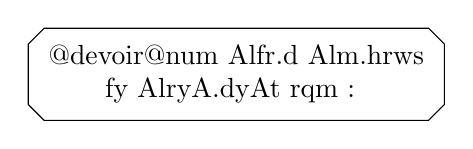
\begin{tikzpicture}
\node [draw,shape=chamfered rectangle] (box2){%
    \begin{minipage}{0.4\textwidth}
       \center\cmdEX@devoir@num \RL{Alfr.d Alm.hrws fy AlryA.dyAt rqm :{} }
    \end{minipage}
};
\end{tikzpicture}%
\else
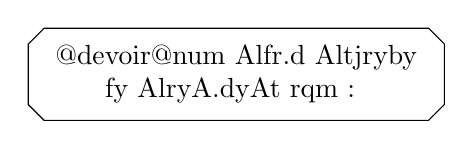
\begin{tikzpicture}
\node [draw,shape=chamfered rectangle] (box2){%
    \begin{minipage}{0.4\textwidth}
       \center\cmdEX@devoir@num \RL{Alfr.d Altjryby fy AlryA.dyAt rqm :{} }
    \end{minipage}
};
\end{tikzpicture}%
\fi
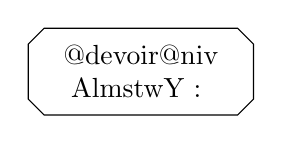
\begin{tikzpicture}
\node [draw,shape=chamfered rectangle] (box3){%
    \begin{minipage}{0.2\textwidth}
 \center\cmdEX@devoir@niv \RL{AlmstwY :{} }     
    \end{minipage}
};
\end{tikzpicture}%
}
%------------------------------------------------\serie[titre=..]-----------------------------------------------------------------------------%

\define@cmdkey[EX]{serie}{titre}{}
\presetkeys[EX]{serie}{titre=\RL{`nwAn Aldrs}}{}
\newcommand{\serie}[1][]{
\setkeys[EX]{serie}{#1}
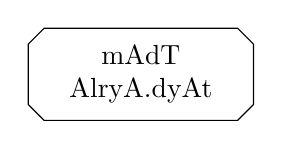
\begin{tikzpicture}
\node [draw,shape=chamfered rectangle] (box1){%
    \begin{minipage}{0.20\textwidth}
       \center\RL{mAdT AlryA.dyAt}
    \end{minipage}
};
\end{tikzpicture}%
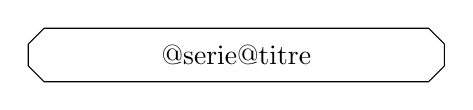
\begin{tikzpicture}
\node [draw,shape=chamfered rectangle] (box2){%
    \begin{minipage}{0.40\textwidth}
      \center\cmdEX@serie@titre
    \end{minipage}
};
\end{tikzpicture}%
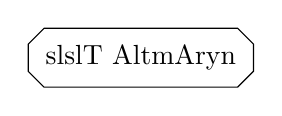
\begin{tikzpicture}
\node [draw,shape=chamfered rectangle] (box3){%
    \begin{minipage}{0.20\textwidth}
   \center\RL{slslT AltmAryn}
    \end{minipage}
};
\end{tikzpicture}%
}
\makeatother

%\cadre[x=0.5,y=0.1,doubleline]

\pagestyle{empty}
\begin{document}
\ExamEntete

\exercice[bareme, bar=4]{
\question[bareme, bar=1.5]{A.hsb w bs.t mA yly :}
$$
A=\left( \dfrac{\sqrt{7}}{\sqrt{3}}\right)^{2}+\left( \dfrac{\sqrt{3}}{\sqrt{5}}\right)^{-2}  
\hspace{0.5cm};\hspace{0.5cm}
B=3\sqrt{75}+2\sqrt{300}-10\sqrt{12}
\hspace{0.5cm};\hspace{0.5cm}
C=\sqrt{10+\sqrt{36}}
$$
\question[bareme, bar=1]{A.h_df Alj_dr Almrb` mn AlmqAm :}
$$
D=\dfrac{2}{\sqrt{11}}
\hspace{0.5cm};\hspace{0.5cm}
E=\dfrac{1}{\sqrt{7}+\sqrt{5}}
$$
\question[bareme, bar=0.5]{A`.t AlktAbT Al`lmyT lil`dad : $F=0.0042 \times 10^{-5}$}
\question[bareme, bar=0.5]{ An^sr mA yly :$G=(\sqrt{3}-a)^{2}+2(1+\sqrt{3}a)$ }
\question[bareme, bar=0.5]{`aml mA yly : $(100-a^{2})+2(10+a)$}
}

\exercice[bareme, bar=5]{
\question[bareme, bar=1]{qArn Al`dadyn $3\sqrt{5}$ w $3\sqrt{7}$ , _tm Astntj mqArnT $5-3\sqrt{5}$ w $5-3\sqrt{7}$ .}
\begin{arabtext}
ltkn $a$ w $b$ w $c$ A`dAd .hqyqyT  .hy_t : $1\leq a \leq 5$ w $3\leq b \leq 4$ w $-5 \leq \dfrac{2c+1}{3} \leq -3$ 
\end{arabtext}
\question[bareme, bar=1.5]{A.tr $a+b$ w $a-b$ w $a\times b$}
\question[bareme, bar=0.5]{byn anna : $-8\leq c \leq -5$}
\question[bareme, bar=2]{A.tr $b^{2}$w $c^{2}$ w $b^{2}\times c$}
}

\exercice[bareme, bar=6]{
\begin{minipage}{0.4\linewidth}
\begin{tikzpicture}[line cap=round,line join=round,>=triangle 45,x=1.0cm,y=1.0cm,rounded corners=0pt]
\clip(-3.34,0.9) rectangle (3.64,5.96);
\draw[line width=1.pt,fill=black,fill opacity=0.10000000149011612] (-0.6860393116298644,1.9622589831573736) -- (-0.6889351603093792,2.245086870856634) -- (-0.9717630480086393,2.2421910221771193) -- (-0.9688671993291248,1.959363134477859) -- cycle; 
\draw (-1.,5.)-- (-2.86,1.94);
\draw  (-2.86,1.94)-- (3.,2.);
\draw  (3.,2.)-- (-1.,5.);
\draw  (-1.,5.)-- (-0.9688671993291248,1.959363134477859);
\begin{scriptsize}
\draw [fill=black] (-1.,5.) circle (2.5pt);
\draw[color=black] (-0.86,5.45) node {$A$};
\draw [fill=black] (-2.86,1.94) circle (2.5pt);
\draw[color=black] (-2.9,2.43) node {$B$};
\draw [fill=black] (3.,2.) circle (2.5pt);
\draw[color=black] (3.14,2.37) node {$C$};
\draw [fill=black] (-0.9688671993291248,1.959363134477859) circle (2.0pt);
\draw[color=black] (-0.8,1.71) node {$H$};
\end{scriptsize}
\end{tikzpicture}
\end{minipage}
\begin{minipage}{0.6\linewidth}
\begin{arabtext}
$( I$n`tbr Al^skl jAnbh , .hy_t $AC=\sqrt{52}$ w $BH=9$ w $HC=4$.
\end{arabtext}
\question[bareme, bar=1]{A.hsb $AH$ w $AB$ .}
\question[bareme, bar=1]{byn An Alm_tl_t $ABC$ qA'im AlzAwyT .}
\question[bareme, bar=1]{A.hsb Alnsb Alm_tl_tyT lilzAwyT $\widehat{ABC}$}
\begin{arabtext}
$( II$ $x$ zAwyT .hAdT b.hy_t : $\sin x =\dfrac{1}{2}$
\end{arabtext}
\question[bareme, bar=1]{A.hsb $\cos x$ w $\tan x$}
\end{minipage}
\question[bareme, bar=1]{bs.t mA yly :
$A = \sin^{2}26^{\circ} +4\cos30^{\circ} +\sin^{2}64^{\circ}-4\sin60^{\circ} $}
\question[bareme, bar=1]{byn anna : $\dfrac{1+\tan^{2}x}{\tan^{2}x}\times (1-cos^{2}x)=1$}
}

\exercice[bareme, bar=3]{
\begin{minipage}{0.4\linewidth}
\begin{tikzpicture}[line cap=round,line join=round,>=triangle 45,x=1.0cm,y=1.0cm,rounded corners=0pt]
\clip(-3.6,1.02) rectangle (5.14,6.86);
\draw  (-2.,6.)-- (-1.56,1.98);
\draw  (4.,2.)-- (-1.56,1.98);
\draw  (4.,2.)-- (-2.,6.);
\draw [domain=-3.6:5.14] plot(\x,{(-19.2708426073132-0.02*\x)/-5.56});
\draw [domain=-3.6:5.14] plot(\x,{(-13.870842607313195--4.*\x)/-6.});
\begin{scriptsize}
\draw [fill=black] (-2.,6.) circle (2.5pt);
\draw[color=black] (-1.86,6.37) node {$A$};
\draw [fill=black] (-1.56,1.98) circle (2.5pt);
\draw[color=black] (-1.46,1.71) node {$C$};
\draw [fill=black] (4.,2.) circle (2.5pt);
\draw[color=black] (4.14,2.37) node {$B$};
\draw [fill=black] (-1.721966491378256,3.459784762137703) circle (2.5pt);
\draw[color=black] (-1.5,3.91) node {$J$};
\draw [fill=black] (1.7913660266601434,3.4724226488932373) circle (2.0pt);
\draw[color=black] (1.94,3.81) node {$K$};
\draw [fill=black] (0.4866674819615999,1.9873621132444659) circle (2.0pt);
\draw[color=black] (0.38,1.75) node {$I$};
\end{scriptsize}
\end{tikzpicture}
\end{minipage}
\begin{minipage}{0.6\linewidth}
\begin{arabtext}
$ABC$ m_tl_t .hy_t $AC=6$ w $CB=9$ w $AJ=4$  w $(BC)//(JK)$
\end{arabtext}
\question[bareme, bar=1.5]{A.hsb AlmsAfT $JK$ .}
\question[bareme, bar=1.5]{$I$ nq.tT mn $[CB] $ b.hy_t : $CI=3$}
\begin{arabtext}
A_tb_t An : $(AB)//(IJ)$
\end{arabtext}
\end{minipage}
}

\exercice[bareme, bar=2]{
\begin{arabtext}
$(C)$ dA'irT mrkzhA $O$ .hy_t $\widehat{ADC}=30^{\circ}$
\end{arabtext}
\question[bareme, bar=1]{A.hsb m`lilA jwAbk qyAs AlzAwyT : $\widehat{ABC}$.}
\question[bareme, bar=1]{A.hsb m`lilA jwAbk qyAs AlzAwyT : $\widehat{AOC}$.}

\begin{center}
\begin{tikzpicture}[line cap=round,line join=round,>=triangle 45,x=1.0cm,y=1.0cm,rounded corners=0pt]
\clip(-7.24,-5.46) rectangle (8.92,8.24);
\draw [shift={(-1.9701425001453319,6.8805700005813275)},line width=1.pt,fill=black,fill opacity=0.10000000149011612] (0,0) -- (-127.98187826603679:0.6) arc (-127.98187826603679:-106.5948402135938:0.6) -- cycle;
\draw (-1.,3.) circle (4.cm);
\draw  (-5.,3.)-- (3.,3.);
\draw  (-5.,3.)-- (-1.9701425001453319,6.8805700005813275);
\draw (-1.9701425001453319,6.8805700005813275)-- (-3.936148830333893,0.28356298690197645);
\draw (-3.936148830333893,0.28356298690197645)-- (-1.,3.);
\draw [line width=1.pt,dash pattern=on 5pt off 5pt] (-3.936148830333893,0.28356298690197645)-- (3.,3.);
\begin{scriptsize}
\draw [fill=black] (-1.,3.) circle (2.5pt);
\draw[color=black] (-1.02,3.51) node {$O$};
\draw [fill=black] (3.,3.) circle (2.5pt);
\draw[color=black] (3.32,3.37) node {$B$};
\draw[color=black] (-3.92,6.65) node {(C)};
\draw [fill=black] (-5.,3.) circle (2.5pt);
\draw[color=black] (-5.3,3.33) node {$C$};
\draw [fill=black] (-3.936148830333893,0.28356298690197645) circle (2.5pt);
\draw[color=black] (-4.36,0.15) node {$A$};
\draw [fill=black] (-1.9701425001453319,6.8805700005813275) circle (2.5pt);
\draw[color=black] (-2.3,7.23) node {$D$};
\draw[color=black] (-2.5,5.8) node {$30^{\circ}$};
\end{scriptsize}
\end{tikzpicture}
\end{center}
}

\RL{.h.z s`yd}

\end{document}